\chapter{TINJAUAN PUSTAKA}
\section{Hasil Penelitian Terdahulu}

\section{Aljabar Max-Plus}
Aljabar max-plus salah satu cabang dari aljabar tropikal yang menggunakan operasi maksimum dan penjumlahan sebagai operasi dasar.
\begin{definisi}[\cite{subiono2015minmaxplus}]
  Aljabar max-plus adalah himpunan $\mathbb{R}_{\max} = \mathbb{R} \cup \{-\infty\}$ yang dilengkapi dengan dua operasi biner yaitu:
  \begin{align*}
    a \oplus b  & = \max\{a, b\}, \quad \forall a, b \in \mathbb{R}_{\max} \\
    a \otimes b & = a + b, \quad \forall a, b \in \mathbb{R}_{\max}
  \end{align*}
  dengan elemen identitasnya adalah $\varepsilon=-\infty$ untuk operasi $\oplus$ dan $0$ untuk operasi $\otimes$.
\end{definisi}

Selanjutnya $(\mathbb{R}_{\max}, \oplus, \otimes)$ disebut sebagai semiring max-plus, yaitu suatu struktur aljabar yang memenuhi sifat seperti ring biasa, kecuali tidak memiliki elemen invers untuk operasi $\oplus$.

\subsection{Matriks Aljabar Max-Plus}
Pada aljabar max-plus, matriks juga dapat didefinisikan dengan menggunakan operasi penjumlahan dan perkalian pada aljabar max-plus. Sebuah matriks bisa dianggap sebagai representasi dari suatu sistem diskrit atau graf berarah berbobot, sehingga dapat digunakan untuk memodelkan berbagai permasalahan matematika \parencite{subiono2015minmaxplus}.
\begin{definisi}[\cite{Baccelli1994maxplus}]
  Misalkan $A = (a_{ij})$ adalah matriks berukuran $m \times n$ dan $B = (b_{ij})$ adalah matriks berukuran $n \times p$ dengan elemen-elemen dari $\mathbb{R}_{\max}$. Operasi penjumlahan dan perkalian matriks pada aljabar max-plus didefinisikan sebagai berikut:
  \begin{align*}
    (A \oplus B)_{ij}  & = a_{ij} \oplus b_{ij} = \max\{a_{ij}, b_{ij}\}                                          \\
    (A \otimes B)_{ij} & = \bigoplus_{k=1}^{n} a_{ik} \otimes b_{kj} = \max_{1 \leq k \leq n} \{a_{ik} + b_{kj}\}
  \end{align*}
\end{definisi}

\begin{contoh}
  Misalkan diberikan matriks $A$ dan $B$ sebagai berikut:
  \[
    A = \begin{pmatrix}
      2 & 3 \\
      5 & 1
    \end{pmatrix}, \quad
    B = \begin{pmatrix}
      4 & 0 \\
      2 & 6
    \end{pmatrix}
  \]
  Maka, penjumlahan dan perkalian matriks $A$ dan $B$ pada aljabar max-plus adalah:
  \begin{align*}
    A \oplus B  & = \begin{pmatrix}
                      \max\{2, 4\} & \max\{3, 0\} \\
                      \max\{5, 2\} & \max\{1, 6\}
                    \end{pmatrix} = \begin{pmatrix}
                                      4 & 3 \\
                                      5 & 6
                                    \end{pmatrix}              \\
    A \otimes B & = \begin{pmatrix}
                      \max\{2 + 4, 3 + 2\} & \max\{2 + 0, 3 + 6\} \\
                      \max\{5 + 4, 1 + 2\} & \max\{5 + 0, 1 + 6\}
                    \end{pmatrix} = \begin{pmatrix}
                                      6 & 9 \\
                                      9 & 7
                                    \end{pmatrix}
  \end{align*}
\end{contoh}

\subsection{Polinomial dalam Aljabar Max-Plus}
Polinomial adalah suatu ekspresi matematika yang terdiri dari variabel dan koefisien, yang dioperasikan dengan penjumlahan, pengurangan, dan perkalian. Dalam aljabar max-plus, polinomial juga dapat didefinisikan dengan menggunakan operasi maksimum dan penjumlahan pada aljabar max-plus \parencite{burden2010numerical}.

\subsection{Matriks Linde-de la Puente}
Berdasarkan hasil penelitian \textcite{linde2014matricescommutinggivennormal}, diperoleh bahwa kekomutatifan antara dua matriks tropikal cukup bergantung pada diagonal utama matriks tersebut. Dalam perkembangan selanjutnya, \textcite{alhussaini2024securityinitialtropical} memperkenalkan juga sebuah protokol kriptografi yang terinspirasi dari pertukaran kunci Diffie-Hellman, yang basisnya adalah grup siklik $(\Z_p^*\ ,\ \times)$ untuk suatu bilangan prima $p$.
\begin{definisi}[Matriks Ldlp]
  Untuk setiap bilangan real $r \leq 0$ dan bilangan real $k \geq 0$, kita definisikan
  $
    [2r, r]_{n}^{k}
  $
  sebagai himpunan matriks $A_{n\times n}$ sedemikian sehingga $a_{ii} = k$ untuk semua $i$ dan $a_{ij} \in [2r, r]$ untuk $i \neq j$.
\end{definisi}
dari definisi di atas diperoleh sebuah teorema penting mengenai kekomutatifan matriks tropikal.
\begin{teorema}
  Misalkan $A \in [2r, r]_{n}^{k_{1}}, \, B \in [2s, s]_{n}^{k_{2}}$ untuk setiap $r, s \leq 0$ dan $a_{ii} = k_{1} \geq 0, \, b_{ii} = k_{2} \geq 0$. Maka
  \[
    A \otimes B = B \otimes A = k_{2} \otimes A \oplus k_{1} \otimes B.
  \]
\end{teorema}

\section{Permutasi}
Dalam aljabar, permutasi ialah suatu fungsi bijektif dari himpunan ke dirinya sendiri. Sebuah permutasi dari himpunan $X = \{1, 2, \ldots, n\}$ biasanya disimbolkan dengan $\sigma: X \to X$, dengan $\sigma$ bersifat satu-satu dan pada. Himpunan semua permutasi dari $X$ membentuk suatu grup terhadap operasi komposisi fungsi, yang disebut grup simetris pada $n$ elemen yang disimbolkan dengan $S_n$ \parencite{subiono2022aljabar}.
\begin{contoh}
  Misalkan diberikan himpunan $X = \{1, 2, 3\}$. Salah satu permutasi dari himpunan $X$ adalah fungsi $\sigma$ yang didefinisikan sebagai berikut:
  \[
    \sigma(1) = 2, \quad \sigma(2) = 3, \quad \sigma(3) = 1
  \]
  atau dapat dituliskan dalam bentuk sebuah matriks berikut
  \[
    \sigma = \begin{pmatrix}
      1 & 2 & 3 \\
      2 & 3 & 1
    \end{pmatrix}
  \]
\end{contoh}
\subsection{Sikel}
Misalkan $\tau$ adalah permutasi pada himpunan $X = \{1,2,\ldots,n\}$.
Untuk suatu elemen $i_1 \in X$, perhatikan barisan
$
  (i_1,\ \tau(i_1),\ \tau^2(i_1),\ \ldots).
$
Karena himpunan $X$ berhingga, terdapat bilangan $k \ge 1$ sehingga
$
  \tau^{k}(i_1) = i_1.
$
Himpunan
\[
  \mathcal{O}_{\tau}(i_1)
  =
  \{\, i_1,\ \tau(i_1),\ \tau^{2}(i_1),\ \ldots,\ \tau^{k-1}(i_1)\,\}
\]
disebut \emph{orbit} dari $\tau$ yang melalui $i_1$.
Orbit menggambarkan lintasan elemen $i_1$ di bawah penerapan berulang dari permutasi $\tau$ \parencite{artin1991algebra}.

\begin{definisi}
  Jika orbit $\mathcal{O}_{\tau}(i_1)$ memuat lebih dari satu elemen, maka orbit tersebut disebut
  \emph{sikel} dari permutasi $\tau$. Dalam notasi siklus, sikel tersebut dituliskan sebagai
  \[
    (i_1\ i_2\ \ldots\ i_k),
  \]
  yang menyatakan bahwa
  \[
    \tau(i_j) = i_{j+1} \quad \text{untuk } 1 \le j < k,
    \qquad
    \tau(i_k) = i_1.
  \]
\end{definisi}

\begin{teorema}[\cite{subiono2022aljabar}]
  Setiap permutasi $\tau\in S_n$ dapat dituliskan sebagai hasil komposisi dari sikel-sikel yang saling asing.
\end{teorema}

Dengan menggunakan notasi sikel, permutasi akan lebih ringkas untuk dituliskan dan dipahami.

\begin{contoh}
  Misalkan diberikan permutasi $\tau\in S_9$ yang didefinisikan
  \begin{align}
    \tau=\begin{pmatrix}
           1 & 2 & 3 & 4 & 5 & 6 & 7 & 8 & 9 \\
           3 & 1 & 2 & 5 & 4 & 6 & 8 & 7 & 9
         \end{pmatrix}.
  \end{align}
  Dengan menggunakan notasi sikel, permutasi $\tau$ dapat dituliskan sebagai
  \[
    \tau = (1\ 3\ 2)(4\ 5)(6)(7\ 8)(9).
  \]
  \begin{figure}[H]
    \centering
    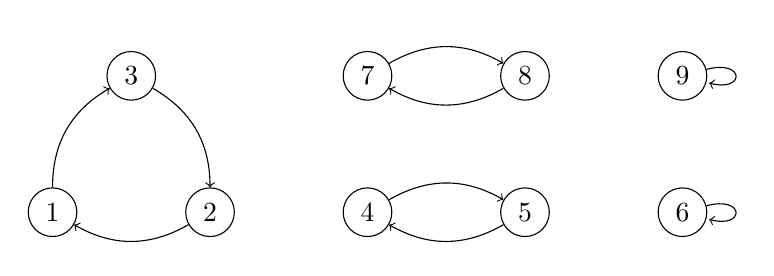
\begin{tikzpicture}[scale=1]
      \node[circle, draw] (1) at (0, 0) {1};
      \node[circle, draw] (2) at (2, 0) {2};
      \node[circle, draw] (3) at (1, 1.732) {3};
      \node[circle, draw] (4) at (4, 0) {4};
      \node[circle, draw] (5) at (6, 0) {5};
      \node[circle, draw] (6) at (8, 0) {6};
      \node[circle, draw] (7) at (4, 1.732) {7};
      \node[circle, draw] (8) at (6, 1.732) {8};
      \node[circle, draw] (9) at (8, 1.732) {9};

      \draw[->] (1) to[bend left] node[above] {} (3);
      \draw[->] (3) to[bend left] node[above] {} (2);
      \draw[->] (2) to[bend left] node[above] {} (1);

      \draw[->] (4) to[bend left] node[above] {} (5);
      \draw[->] (5) to[bend left] node[above] {} (4);

      \path (6) edge[->, loop right] ();

      \draw[->] (7) to[bend left] node[above] {} (8);
      \draw[->] (8) to[bend left] node[above] {} (7);

      \path (9) edge[->, loop right] ();
    \end{tikzpicture}
    \caption{Diagram sikel dari permutasi $\tau$}
    \label{fig:sikel}
  \end{figure}
\end{contoh}

\subsection{Matriks Permutasi}
Setiap permutasi $\sigma \in S_n$ dapat kita representasikan dalam bentuk matriks permutasi $P_{\sigma}\in\R^{n \times n}$ yang elemen-elemennya hanya terdiri dari $0$ dan $1$, dengan aturan sebagai berikut:
\[
  (P_{\sigma})_{ij} =
  \begin{cases}
    1, & \text{jika } i = \sigma(j), \\
    0, & \text{lainnya}.
  \end{cases} \quad \forall i, j = 1, 2, \ldots, n.
\]
Dalam konteks aljabar max-plus, matriks permutasi juga dapat didefinisikan dengan cara yang serupa, di mana elemen-elemen matriks hanya terdiri dari $-\infty$ dan $0$ yang merepresentasikan identitas dan elemen nol dalam aljabar max-plus.
\begin{definisi}[\cite{Farlow2009}]
  Misalkan $\sigma : \{1,2,\dots,n\} \to \{1,2,\dots,n\}$
  adalah suatu permutasi, maka matriks permutasi max-plus
  $P_{\sigma} = [p_{ij}]$ didefinisikan sebagai
  \[
    p_{ij} =
    \begin{cases}
      0,       & \text{jika } i = \sigma(j), \\[4pt]
      -\infty, & \text{lainnya}.
    \end{cases}
  \]
\end{definisi}

\begin{contoh}
  Misalkan diberikan permutasi $\sigma=(1\ 3\ 2)\in S_3$. Maka, matriks permutasi max-plus $P_{\sigma}$ adalah
  \[
    P_{\sigma} =
    \begin{pmatrix}
      -\infty & -\infty & 0       \\
      0       & -\infty & -\infty \\
      -\infty & 0       & -\infty
    \end{pmatrix}.
  \]
\end{contoh}

\begin{teorema}[\cite{Farlow2009}]
  Sebuah matriks $A \in \mathbb{R}_{\max}^{n \times n}$ memiliki invers kanan
  jika dan hanya jika terdapat suatu permutasi $\sigma$ serta nilai-nilai
  $\lambda_i > \varepsilon$, $i \in \{1,2,\dots,n\}$, sehingga
  \[
    A = P_{\sigma} \otimes D(\lambda).
  \]
\end{teorema}


\section{\textit{Latin Square}}
\textit{Latin square} adalah susunan $n \times n$ larik yang diisi dengan $n$ simbol berbeda, sehingga setiap simbol muncul tepat satu kali pada setiap baris dan setiap kolom.
Pertama kali diperkenalkan oleh Leonhard Euler pada abad ke-18 dalam konteks teka-teki matematika tentang ``\textit{36 military officers}'' \parencite{george2017introductioncombinatorics}.


